\documentclass{beamer}
%\documentclass[notes=only]{beamer}
\usepackage[utf8x]{inputenc}
\usepackage[ngerman]{babel}
\usetheme{Bergen}
\usepackage{tikz}
\usepackage{listings}
\usepackage{chronology}

\title{Analyse einer historischen Musikzeitung}
\author{Bettina Riedl}
\begin{document}
\begin{frame}[plain]
    \maketitle
\end{frame}
\note{}
\begin{frame}{Idee: klassische Musik}
	\begin{itemize}
		\pause
		\item Vorteil: Quellen ohne Copyright
		\pause
		\item historische, musikalische Zeitschrift analysieren
		\pause
		\item Spotify Api für Verlgeichsdaten aus der Gegenwart
		\pause
		\item Wikipedia \glqq Liste klassischer Komponisten\grqq als Schlagwortverzeichnis
	\end{itemize}
\begin{block}{Fragestellungen}
	\begin{itemize}
		\item Welche Komponisten werden überproportional oft genannt?
		\item Welche Komponisten, die zu bestimmten Zeiten berühmt waren, sind heutzutage nicht mehr populär?
		\item Welche Komponisten werden oft in einem Absatz zusammen genannt?
	\end{itemize}
\end{block}
\end{frame}
\note[itemize]{
	\item keine Ahnung von bildender Kunst
}
\begin{frame}{Allgemeine Musikalische Zeitung}
	\begin{itemize}
		\item wöchentliche Zeitschrift
		\item erschienen 1798–1848 und 1863-1882,  meist im Verlag \glqq Breitkopf \& Härtel Verlag\grqq
		\item vollständige, hochqualitative Scans einer Jahresauflage auf Google Books downloadbar
		\item 1 Band $\widehat{=}$ 52 Ausgaben $\approx$ 500 Seiten\\
		70 Bände $\approx$ 35 000 Seiten
		\item Inhalt: Rezensionen, Anekdoten
	\end{itemize}
\end{frame}
\note{
	Musikelische Zeitung deckt Zeit des Bidermeiers/Frühromantik bis Spätromantik -> nachvollziehung der Entwicklung der Popuiarität einzelner Künstler}
\begin{frame}{Zeitstrahl}
	\begin{tikzpicture}[scale=0.88]
		\draw[->] (-1.1, 4) -- (9, 4);
		\node[below] at (0, 4) {1750};
		\node[below] at (1.5, 4) {1775};
		\node[below] at (3, 4) {1800};
		\node[below] at (4.5, 4) {1825};
		\node[below] at (6, 4) {1850};
		\node[below] at (7.5, 4) {1875};
		\node[below] at (9, 4) {1900};

		\pause
		
		\draw[rounded corners] (-1.08, 4.2) rectangle (3.54, 4.7) node[midway] {Joseph Haydn};
		%\node at (0, 5) {};
		
		\draw[rounded corners] (0.36, 4.8) rectangle (2.46, 5.3) node[midway] {Mozart};
		
		%Beethoven
		\draw[rounded corners] (1.2, 5.5) rectangle (4.62, 6) node[midway] {L.v.Beethoven};
		
		\pause
		
		% Schubert
		\draw[rounded corners] (2.82, 6.2) rectangle (4.68, 6.7) node[midway] {Schubert};
		
		% Robert Schumann
		\draw[rounded corners] (3.6, 6.9) rectangle (6.36, 7.4) node[midway] {R. Schumann};
		
		% Frederic Chopin
		\draw[rounded corners] (3.6, 7.6) rectangle (5.94, 8.1) node[midway] {F. Chopin};
		
		% Franz Liszt
		\draw[rounded corners] (3.66, 8.3) rectangle (8.16, 8.8) node[midway] {Franz Liszt};
		
		% Richard Wagner
		\draw[rounded corners] (3.78, 9) rectangle (7.98, 9.5) node[midway] {Richard Wagner};
		
		\pause
		
		\draw[rounded corners] (2.88, 3.4) rectangle (5.88, 2.9) node[midway] {AMZ};
		\draw[rounded corners] (6.72, 3.4) rectangle (7.92, 2.9) node[midway] {AMZ};
	\end{tikzpicture}
\end{frame}
\note[itemize]{
	\item zwischen 1848 und 1863 nicht erschienen, da laut der 
}
\begin{frame}{Adieu: 1848}
	 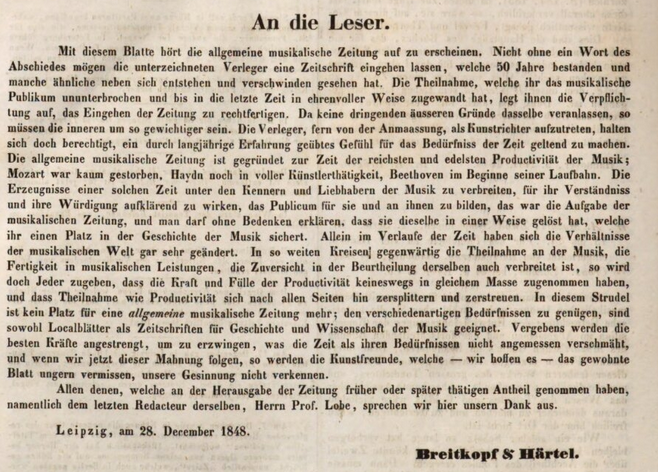
\includegraphics[scale=.39]{"data/adieu.png"}
\end{frame}
\begin{frame}
	\begin{block}{Begründung}
	\begin{itemize}
		\item Gründung der Zeitung während \glqq Zeit der reichsten und edelsten Produktivität\grqq (Wiener Klassik)
		\item mehr Interesse an Musik
		\item weniger \glqq Kraft und Fülle der Produktivität\grqq
		\item zu viel Zersplitterung für eine \glqq allgemeine musikalische Zeitung\grqq
	\end{itemize}
	\end{block}
\end{frame}
\note{1843: Gründung des \glqq Conservatorium der Musik\grqq  in Leipzig durch Felix Mendelson Batholdy}
\begin{frame}
	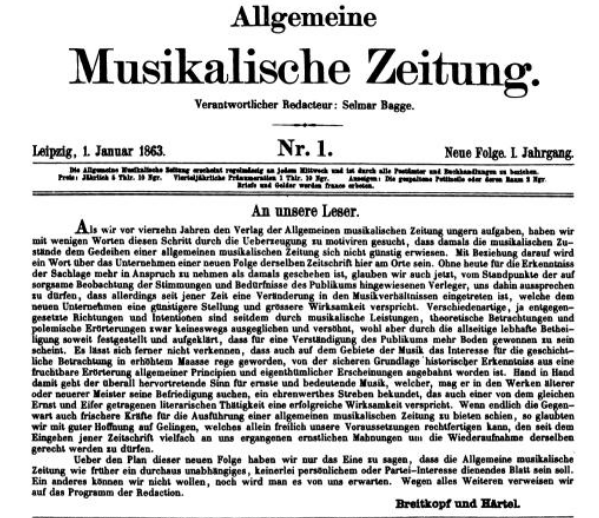
\includegraphics[scale=.43]{"data/hello.png"}
\end{frame}
\begin{frame}
	\begin{itemize}
		\item durch \glqq musikalische Leistung, theoretische Betrachtung und polemische Erörterung" Struktur in verschiedenen Strömungen
		\item geschichtliche, ernste, teilweise fast philosophische Auseinandersetzungen als Themen der Musik
		\item \glqq frische Kräfte für die Ausführung einer allgemeinen musikalischen Zeitung\grqq
		\item Unfähigkeit von einem \glqq freien Standpunkt\grqq über gegenwärtige Musik zu urteilen
	\end{itemize}
\end{frame}
\begin{frame}{Weitere Fragestellungen}
	  	\begin{itemize}
	  		\item Wie gehen die älteren Ausgaben und jüngere Ausgaben mit ihrer gegenwärtigen Musik um?
	  		\item Ausreißer analysieren: Korellation mit  Veröffentlichung berühmter Werke(z.B. durch Spotify Popularität ermittelt)
	  		
	  	\end{itemize}
\end{frame}
\note{mehr qualitative Fragestellungen}
\begin{frame}{Rohmaterial: AMZ Scans}
	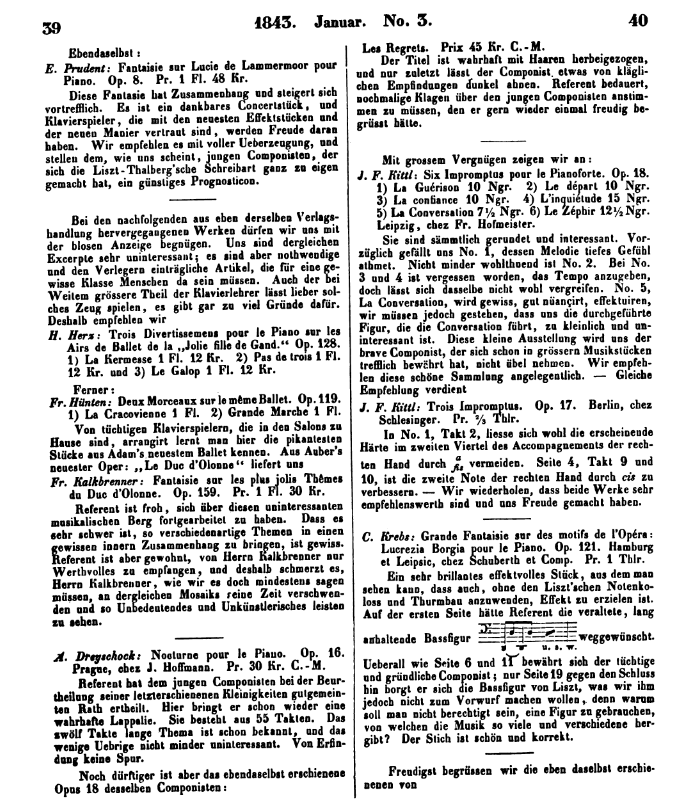
\includegraphics[scale=.29]{"data/amzscreenshot.png"}
\end{frame}
\begin{frame}{Rohmaterial: Wikipedia}
	\begin{itemize}
		\item \glqq Liste von Komponisten klassischer Musik\grqq
		\item MediaWiki Api
		\item Pyton Bib: wikipediaapi
	\end{itemize}
~\\
	
\includegraphics[scale=.21]{"data/wikiKomponistenListe.png"}
	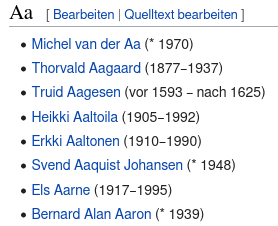
\includegraphics[scale=.3]{"data/wikiKomponistenA.png"}
\end{frame}
\note{ich weiß dass dadurch die Gefahr besteht, dass ein Komponist, der so unbekannt ist, dass er keinen Wikipedia Artikel hat hier übersehen wirds}
\begin{frame}{Rohmaterial: Spotify Daten}
	\begin{itemize}
		\item Spotify Web Api
		\item Python Bib: spotipy
	\end{itemize}
	
\includegraphics[scale=.4]{"data/spotifyscreenshot.png"}
\end{frame}
\begin{frame}{Konzept}
	\begin{block}{\\~\\Preprocessing\\~\\Texterkennung/\\Parsen\\~\\~\\~\\NLP\\~\\Datenanalyse\\~\\Präsentation}
		
		\begin{tikzpicture}[scale=.8]
			
			\node[above] at (0, 8.1)  (amz) {AMZ Scans};
			\node[above] at (3.3, 8)  (wiki) {Wikipedia Artikel};
			\node[above] at (7, 8) (spotify) {Spotify Web Api};
			
			\pause
			
			\draw[->]  (amz) --  (0, 5) node[below] (exText) {extrahierter Text}; 
			
			\pause
			
			\draw[->] (wiki) --  (5.25, 6.5) node[below]  (listComp) {List[Composer]};
		\end{tikzpicture}
	\end{block}
\end{frame}
\begin{frame}{Schnittstelle: \glqq Composer\grqq Klasse}
	\begin{block}{Attribute}
		\begin{itemize}
		\item Vorname
		\item Nachname
		\item Geburtsjahr
		\item Todesjahr
		\item Jahr
		\item spotify\_id
		\item popularity\_spotify
		\item follower\_spotify
	\end{itemize}
	\end{block}
	\begin{block}{Methoden}
		\begin{itemize}
	\item match
\end{itemize}
\end{block}
\end{frame}
\begin{frame}{Konzept}
	\begin{block}{\\~\\Preprocessing\\~\\Texterkennung/\\Parsen\\~\\~\\~\\NLP\\~\\Datenanalyse\\~\\Präsentation}

			\begin{tikzpicture}[scale=.8]

			\node[above] at (0, 8.1)  (amz) {AMZ Scans};
			\node[above] at (3.3, 8)  (wiki) {Wikipedia Artikel};
			\node[above] at (7, 8) (spotify) {Spotify Web Api};
	
			\draw[->]  (amz) --  (0, 5) node[below] (exText) {extrahierter Text}; 
			
			\draw[->] (wiki) --  (5.25, 6.5) node[below]  (listComp) {List[Composer]};
			
			\pause

			\draw[->] (listComp)  -- (spotify);
			
			\pause
			
			\draw[->] (spotify) -- (7, 5) node[below, text width=1cm,align=center] (artistList) {isSpotifyArtist( List[Composer])};
			
			\pause
			
			\node at  (3.5, 3) (datensatz) {Datensatz};
			\draw[->] (artistList) -- (datensatz);
			\draw[->] (exText) -- (datensatz);
			
			\pause
			
			\node at (3.5 , 1.5) (infos) {Informationen};
			\draw[->] (datensatz) -- (infos);
			
			\pause
			
			\node at (3.5, 0) (pres) {Interpretation, Präsentation};
			\draw[->] (infos) -- (pres);
		\end{tikzpicture}
	\end{block}
\end{frame}

\begin{frame}{Parsen der Wikipediadaten}
	\begin{itemize}
		\item $ \left\langle Vorname\right\rangle ^* $   $\left\langle Nachname\right\rangle$ $(\left\langle Geburtsjahr\right\rangle$ - $\left\langle Todesjahr\right\rangle )$
		\item (* 1946)
		\item (frühes 16. Jahrhundert)
		\item (um 1580 bis nach 1629)
		\item (?–1597)
		\item Albertine Morin-Labrecque (auch: Labrecque-Morin, geb. Labrecque, 1886–1957)
		\item Léo-Pol Morin (Pseudonym: James Callihou, 1892–1941)
		\item Franz Joseph Leonti Meyer von Schauensee 
	\end{itemize}
\end{frame}
\begin{frame}{Parsen der Wikipediadaten}
	\begin{itemize}
			\item Regulärer Ausdruck zum Parsen von Name und Geburtsdatum
			\item[$\rightarrow$ ] manuelle Verfeinerung der Regulären Ausdrücke
			\item[Beispiel   ] $ \setminus s^*(um|\sim |vor|nach| \approx )?\setminus s^*(?P\left\langle birth\right \rangle \setminus d\{4,4\})(\setminus?)? $
	\end{itemize}
\end{frame}
\note{aufspalten des Problem in einzelne Reguläre ausdrücke }
\begin{frame}{Vorverarbeitung von AMZ Scanns: Binarisierung und Rauschunterdrückung}
	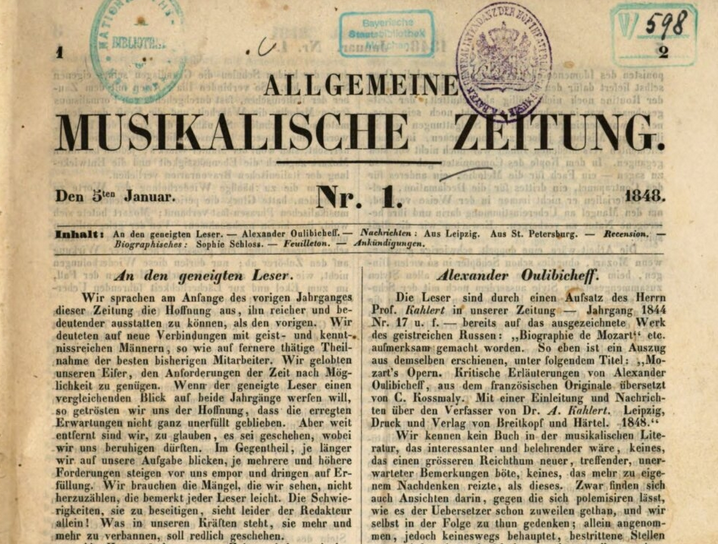
\includegraphics[scale=.36]{"data/unbinarisiert.png"}
\end{frame}
\begin{frame}{Vorverarbeitung von AMZ Scanns: Binarisierung und Rauschunterdrückung}
	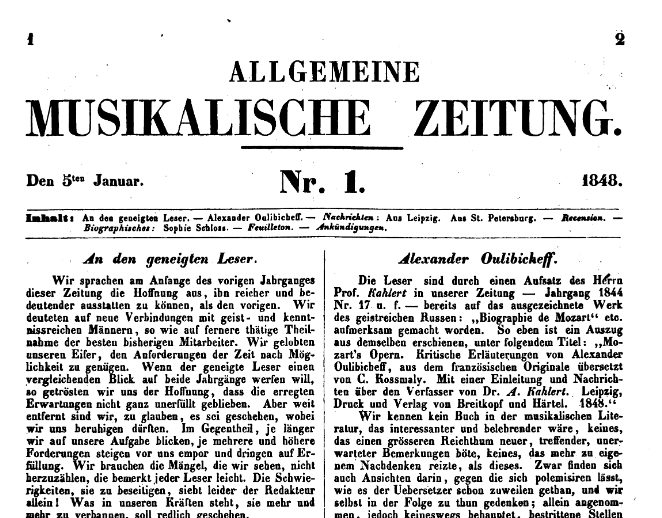
\includegraphics[scale=.38]{"data/processed.png"}
\end{frame}
\note{Schwellenwertverfahren (engl. Thresholding)
	
	
	
	unpaper? binarization schon von google vorgenommen
	google header entfernen}
\begin{frame}{Preprocessing von AMZ Scanns: Binarisierung und Rauschunterdrückung}
	\begin{itemize}
		\item Google Scans sind vorverarbeitet
		\item unpaper: Kommandozeilenprogramm zum Post-Processing
	\end{itemize}
\end{frame}
 \note[itemize]{
\item unpaper scannt eine Seite nach einem Testblock und reduziert dann das Rauschen um diesen Textblock und richtet ihn gerade aus
\item unpaper hat bei mir nicht gut funktioniert, trotz ausprobieren unterscheidlicher einstellungen
}
\begin{frame}{Texterkennung: Tesseract}
\begin{itemize}
		\item Bibliothek fürTexterkennung(engl. optical character recognition, OCR)
		\item künstliche neuronale Netze
		\item freie Software, von Google verwaltet und weiterwentwickelt
		\item bestehende Modelle trainierbar mit eigenen Trainingsdaten
		\item ....txt: \glqq  die Art der Darstellung selbst solcher klei-\grqq \\....tif:
	\end{itemize}
\includegraphics[scale=.5]{"/home/betti/culturalDataScience/venv/lib/tesstrain/script_whole_pages/images/amzText3-027.exp0.png"}
\end{frame}
\begin{frame}{Tesseract Training}
	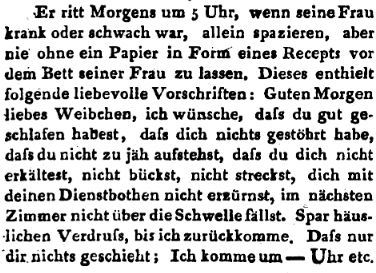
\includegraphics[scale=.6]{"data/tesseractmodelcomp.png"}
\end{frame}
\begin{frame}{Tesseract Training}
	\fontsize{9pt}{10pt}\selectfont
	\begin{block}{\glqq deu\grqq Model}
			\begin{minipage}[t]{0.9\textwidth}
			‘Z.  \\                                             
			~\\   
			dem\textbf{ Bett }seiner Frau zu lassen. Dieses enthielt   \\
			folgende liebevolle Vorschriften: Guten Morgen    \\
			\textbf{J@iebes} \textbf{Weibehen}, ich wünsche, \textbf{dafß }du gut ge-    \\
			schlafen habest,\textbf{ daßfß} dich nichts gestöhrt habe, \\
			\textbf{daß} du nicht zu jäh aufstehst, \textbf{dafßs }du dich nicht\\
			erkältest, nicht bückst, nicht streckst, dich mit \\
			deinen\textbf{ Dienstbethen} nicht erzürnst, im nächsten   
		\end{minipage}
	\end{block}

	\begin{block}{\glqq amz\_trained\grqq\\Model  }
		nach Training mit etwa 150 Trainigszeilen:\\
		~\\
	\begin{minipage}[t]{0.9\textwidth}
		‘“Z.       \\                                       
		~\\ 
		dem \textbf{BEett} seiner Frau zu lassen. Dieses enthielt  \\
		folgende liebevolle Vorschriften: Guten Morgen    \\
		\textbf{liebes}\textbf{ Weibehen}, ich wünsche, \textbf{dafs} du gut ge-     \\
		schlafen habest,\textbf{ dafs} dich nichts gestöhrt habe,  \\
		\textbf{dafs} du nicht zu jäh aufstehst, \textbf{dafs} du dich nicht\\
		erkältest, nicht bückst, nicht streckst, dich mit \\
		deinen \textbf{Dienstbothen} nicht erzürnst, im nächsten 
	\end{minipage}
	\end{block}
\end{frame}
\note[itemize]{
\item nach training immer noch Fehler
\item für bessere Erkennung wsl noch viel mehr trainingsdaten nötig besonders für z.B. zahlen oder sonderzeichen
\item Problem scharfes s als fs geschrieben
}
\begin{frame}{Named Entity Recogition}
	\begin{block}{Fragestellung}
		Wie erkenne ich, dass ein Wort ein Name einer Person/Organisation/Unternehmen ist?
	\end{block}

\end{frame}
\begin{frame}{Ergebnis einer trivialen NER}
	Ge\\
	Re\\
	He\\
	Herr\\
	Kunst\\
	Mozart\\
	Grund\\
	Geist\\
	Su\\
	Schul\\
	Meister\\
	Besch\\
	Finger\\
	Wert\\
	Theile\\
	Tod\\
	Reich\\
\end{frame}
\note{sehr viele falsch Positive}
\begin{frame}{NER Probleme am Beispiel "Bach"}
	\begin{itemize}
		\item \glqq himmelweit von der eines Em. Bach verschieden\grqq
		\item \glqq verdienten Bachischen Hause Uebergebliebenen\grqq
		\item \glqq jungsten Tochter Sebastian Bachs, ist vom Publikum\grqq
		\item \glqq unmitteibarer Schule von Joh. Sebast. Bach,\grqq
		\item \glqq s1. C.P. E Bach in Hamburg\grqq
		\item \glqq L. S Bach\grqq
		\item \glqq  In hetler Fluth der Bach\grqq
		\item \glqq Hier hat Vater Bach denn\grqq
	\end{itemize}
\end{frame}
\note[itemize]{
\item 	verschiedene Komponisten mit gleichem Namen, bekannte Komponisten oft ohne Vornamen
\item schwieirige Lemmatisierung: "Bachsche", "Bachisch", "S. Bach", "J. S. Bach", 
\item Homonyme: Bach Künstler als auch "kleiner natürlicher Wasserlauf von geringer Tiefe und
\item keine moderne, einheitliche Rechtsschreibung
}
\begin{frame}{spaCy}
	\begin{itemize}
		\item Open Source Library für Natural Language Processing in Python
		\item künstlichen neuronalen Netze, trainierbar
	\end{itemize}
\begin{block}{Probleme}
	\begin{itemize}
	\item altdeutsche Rechtschreibung
	\item Formatierung
	\item[$\rightarrow $ ] viele falsch Negative und einige falsch Positive
	\end{itemize}
\end{block}
\end{frame}
\begin{frame}{Schnittstellen}
	content...
\end{frame}
\begin{frame}{Data Mining}
\end{frame}
\begin{frame}{Nächste Schritte}
	\begin{itemize}
		\item Konzentration auf Inhaltsverzeichnis oder Register
		\item tesseract trainieren: altdeutsche Rechtschreibung, Umlaute, Zahlen
		\item spaCy trainieren: altdeutsche Rechtschreibung, konkrete Beipsiele aus extrahiertem Text
		\item 

	\end{itemize}
\end{frame}
\end{document}
